\documentclass[12pt,a4paper]{article}

\usepackage[margin=1in]{geometry}
\usepackage[T1]{fontenc}
\usepackage[utf8]{inputenc}
\usepackage{bookman}
\usepackage{graphicx}
\usepackage{float}
\usepackage{array}
\usepackage{booktabs}
\usepackage{longtable}
\usepackage{enumitem}
\usepackage[hidelinks]{hyperref}
\usepackage{caption}
\usepackage{xcolor}
\usepackage{setspace}
\usepackage{fancyhdr}
\usepackage{titlesec}

\graphicspath{{ui_screenshots/selected/}}
\onehalfspacing

\definecolor{blocpurple}{HTML}{7C3AED}
\definecolor{blocsoftpurple}{HTML}{EDE9FE}
\definecolor{bloctext}{HTML}{111111}
\definecolor{blocmuted}{HTML}{6B7280}

\pagestyle{fancy}
\fancyhf{}
\lhead{\small Bloc -- UI, Database and Code Design Report}
\rhead{\small USIU-Africa, 2026}
\cfoot{\thepage}

\titleformat{\section}
  {\normalfont\Large\bfseries\color{bloctext}}
  {\thesection}{1em}{}
\titleformat{\subsection}
  {\normalfont\large\bfseries\color{bloctext}}
  {\thesubsection}{1em}{}

\captionsetup{
  font=small,
  labelfont=bf,
  justification=centering
}

\setlist[itemize]{leftmargin=1.2cm}
\setlist[enumerate]{leftmargin=1.2cm}

\begin{document}

\begin{titlepage}
    \centering
    \vspace*{1.0cm}
    {\Huge\bfseries BLOC\par}
    \vspace{0.35cm}
    {\Large A Social-First Unified Payments Platform for the Kenyan Market\par}
    \vspace{1.2cm}
    {\Large\bfseries SWE 3090XA User Interface, Database and Code Design Report\par}
    \vspace{1.4cm}

    \begin{tabular}{>{\bfseries}r l}
        Student Name: & Nixon Wainaina \\
        Registration Number: & 665507 \\
        Supervisor: & Ogore.F, Prof \\
        Programme: & BSc Software Engineering \\
        Submission Date: & June 2026 \\
    \end{tabular}

    \vfill
    {\large United States International University -- Africa\par}
    {\large School of Science and Technology\par}
    {\large Nairobi, Kenya\par}
\end{titlepage}

\pagenumbering{roman}

\section*{Declaration}
I, Nixon Wainaina, declare that this report titled \textit{Bloc: User Interface, Database and Code Design Report} is my original work and has not been submitted for examination in any other institution. All sources used to support the design, implementation and analysis have been acknowledged in the references section.

\vspace{1cm}
\noindent Signature:\hrulefill

\vspace{0.4cm}
\noindent Name: Nixon Wainaina

\vspace{0.4cm}
\noindent Date:\hrulefill

\section*{Abstract}
Bloc is a social-first payments platform designed for the Kenyan market. The project responds to a gap in current digital payment experiences: money moves quickly through existing rails, but the user experience often lacks identity, social context, merchant presence and emotional feedback. Bloc introduces human-readable handles, social transaction context, customer profiles and merchant storefronts on top of familiar mobile-money behaviour.

This report follows the SWE 3090XA user interface, database and code design template. It evaluates the current Bloc frontend prototype, explains the design language and navigation model, analyses the modular React code structure, proposes a database model for customers, merchants, handles, transactions and storefront artefacts, and discusses how the interface will integrate with future backend services such as authentication and M-Pesa Daraja API payment routing. Selected screenshots from the current UI are included to demonstrate the strongest visual outcomes of the implementation.

\newpage
\tableofcontents
\newpage
\listoffigures
\newpage

\pagenumbering{arabic}

\section{Introduction}

\subsection{Purpose of the Report}
The purpose of this report is to document and evaluate the Bloc frontend prototype from three connected perspectives: user interface design, database design and code design. The report explains how the interface communicates Bloc's product idea, how the codebase is structured for maintainability, and how the data model can support the social-payment interactions described in the project proposal.

Bloc is not intended to replace M-Pesa. Instead, it is designed as a human layer above payment infrastructure. The product gives people and businesses recognizable identities through @handles, profile pages, transaction notes, merchant storefronts and social payment flows. This report therefore studies both the visible interface and the technical structure required to make that experience reliable.

\subsection{Scope}
The scope of this report covers:
\begin{itemize}
    \item user interface evaluation of the implemented Bloc screens;
    \item responsiveness across mobile and laptop layouts;
    \item code modularity, routing and component separation in the React frontend;
    \item proposed database entities and relationships for the Bloc product domain;
    \item integration points between the frontend, backend services and M-Pesa payment infrastructure;
    \item recommendations for accessibility, testing, security and future backend integration.
\end{itemize}

Backend implementation is outside the current prototype phase. Forms validate locally, routes are client-side and payment actions are intentionally simulated until API integration is introduced.

\subsection{Target Audience}
The target audience for this report includes software engineering assessors, frontend developers, backend developers, UI/UX designers and project stakeholders. The report is written to make the current design understandable enough for evaluation and structured enough for further implementation.

\section{User Interface Analysis}

\subsection{Design Direction}
Bloc's interface follows a social-first design direction. The pages are intentionally clean, image-rich and rounded. The visual system uses a white background, black primary text, muted secondary text, light gray cards and soft purple interactive states. This keeps attention on the people, merchants and transaction context rather than on decorative backgrounds.

The typography choice is Gabarito in the product implementation. It gives the interface a friendly but confident identity. In the LaTeX report, the template-inspired Bookman style is used for academic presentation, while the UI itself preserves the Bloc product typography.

\subsection{Layout and Navigation}
The interface is organized around clear user paths:
\begin{itemize}
    \item the root page lets the visitor choose between customer and merchant onboarding;
    \item customer onboarding focuses on claiming a memorable @handle;
    \item merchant onboarding focuses on business dignity, storefront setup and payout routing;
    \item customer home combines balance, search, social feed and recent transactions;
    \item merchant home summarizes earnings and incoming payments;
    \item profile pages combine identity and payment in one destination;
    \item settings keeps product voice while exposing account, money, notification and privacy controls.
\end{itemize}

Navigation is implemented using React Router. During inspection, protected route blocking was disabled so all pages can be reviewed directly. In a production build, protected routes should redirect unauthenticated users to the landing page, as specified in the design document.

\subsection{Selected Interface Screens}
All current UI routes were captured during this report pass. Only the strongest screenshots are included below so that the report demonstrates quality rather than volume.

\begin{figure}[H]
    \centering
    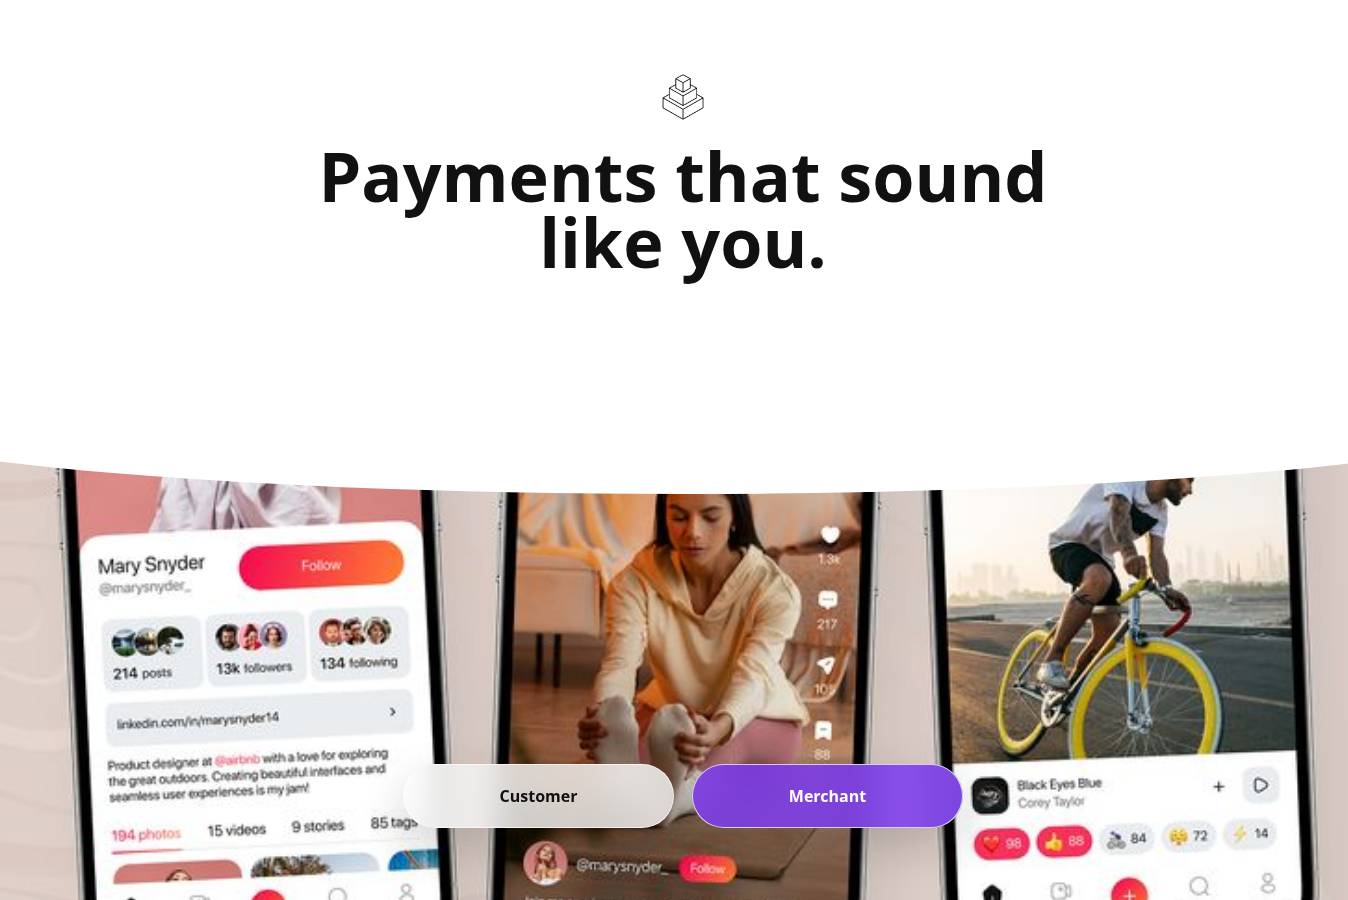
\includegraphics[width=\textwidth]{signup_laptop.png}
    \caption{Bloc root page showing the onboarding split between customer and merchant paths.}
    \label{fig:signup}
\end{figure}

Figure~\ref{fig:signup} shows the first-contact experience. The large headline communicates the central product idea quickly, while the full-bleed image and frosted pill buttons make the page feel like an entrance rather than a static information page.

\begin{figure}[H]
    \centering
    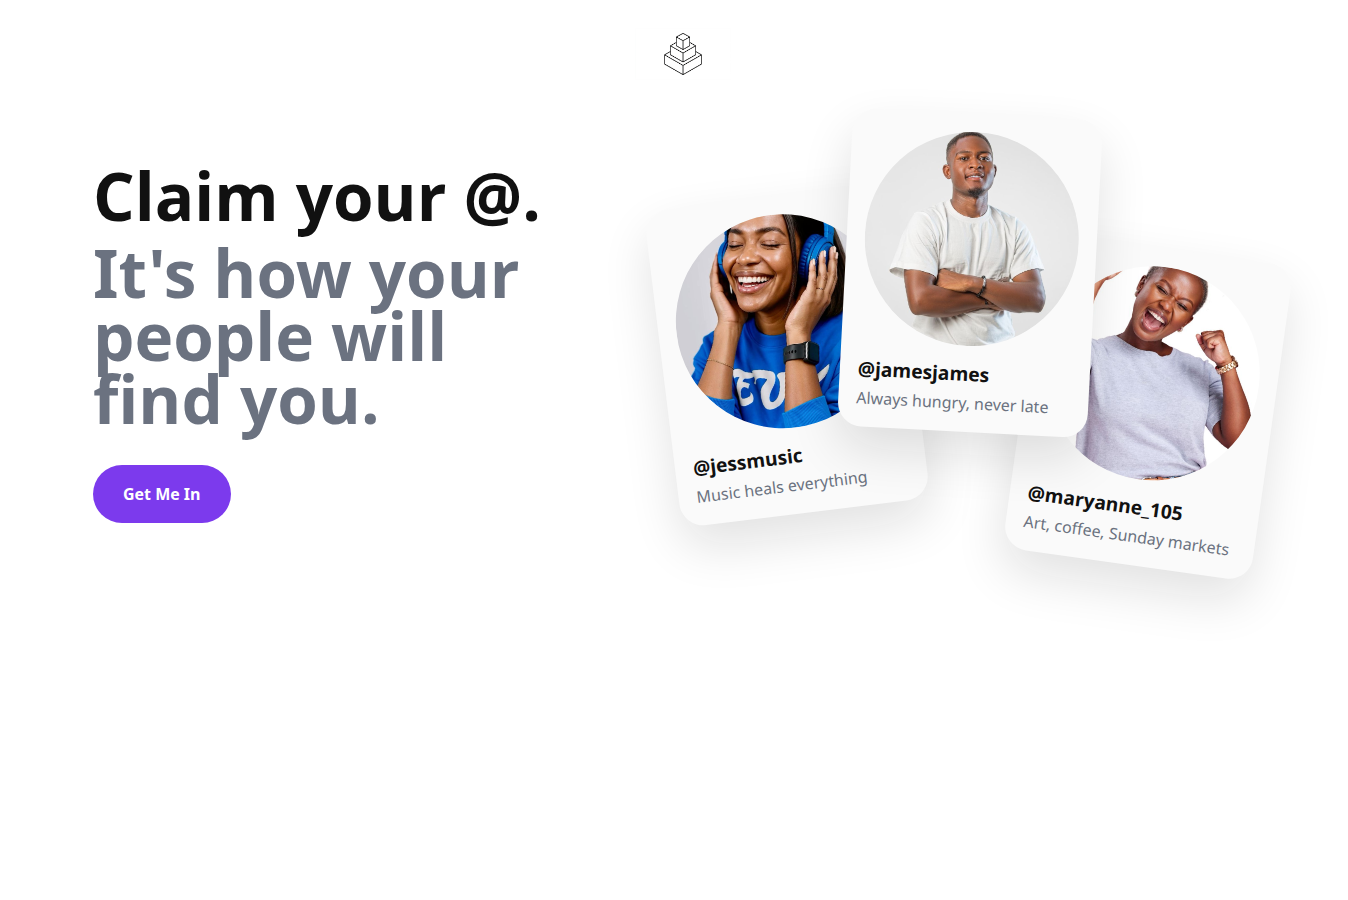
\includegraphics[width=\textwidth]{customer_login_laptop.png}
    \caption{Customer onboarding page emphasizing handle-based identity and social proof.}
    \label{fig:customer-login}
\end{figure}

Figure~\ref{fig:customer-login} demonstrates the social identity concept. Tilted profile cards show that Bloc accounts are people with faces, handles and short biographies, not just phone numbers.

\begin{figure}[H]
    \centering
    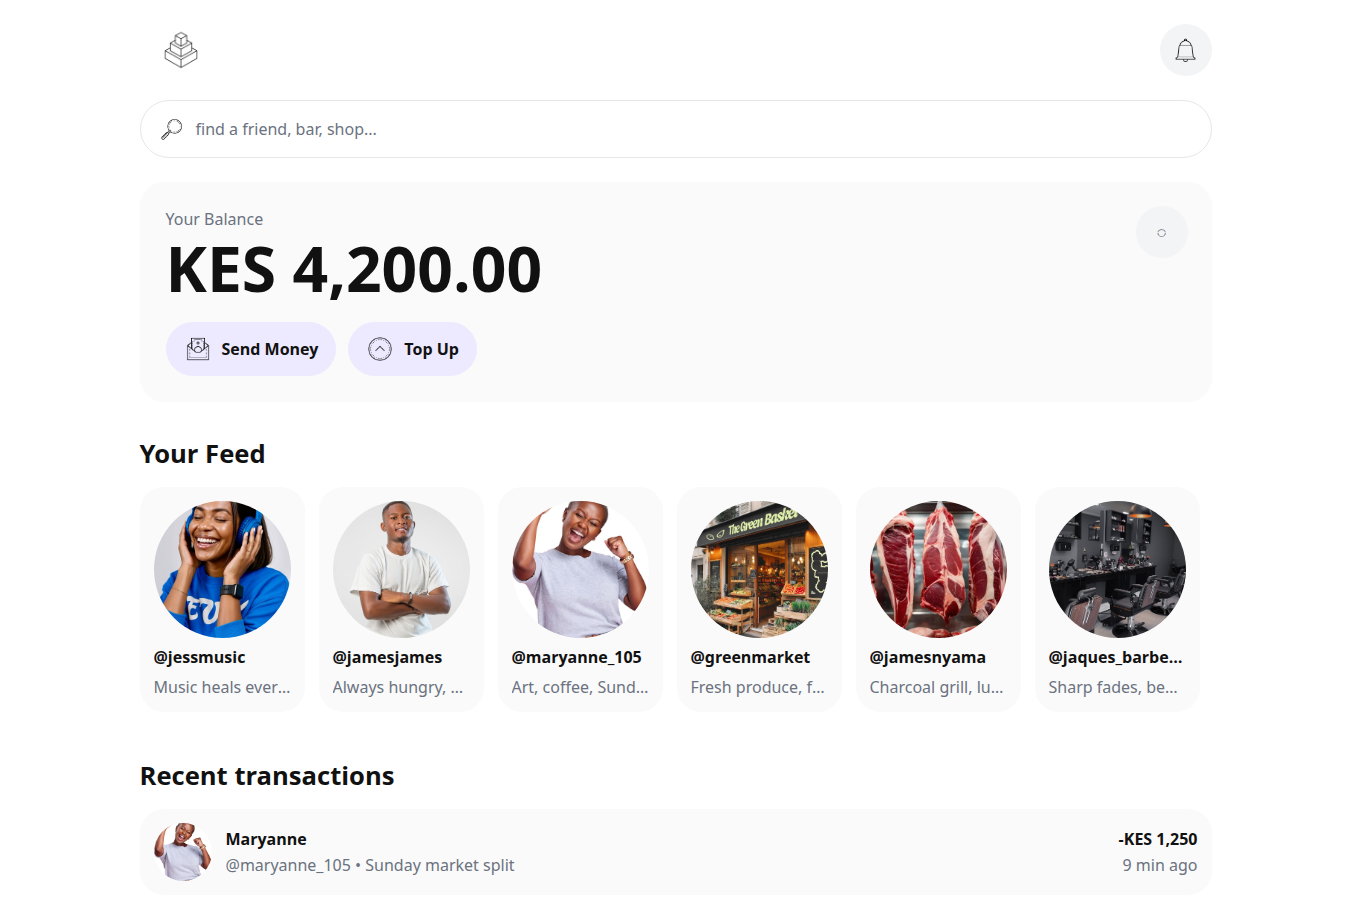
\includegraphics[width=\textwidth]{customer_home_laptop.png}
    \caption{Customer home page with balance, search, social feed and recent transactions.}
    \label{fig:customer-home}
\end{figure}

Figure~\ref{fig:customer-home} shows the customer dashboard. It combines financial utility with social context: balance and payment actions are prominent, while the feed and transaction list make money movement feel connected to people and places.

\begin{figure}[H]
    \centering
    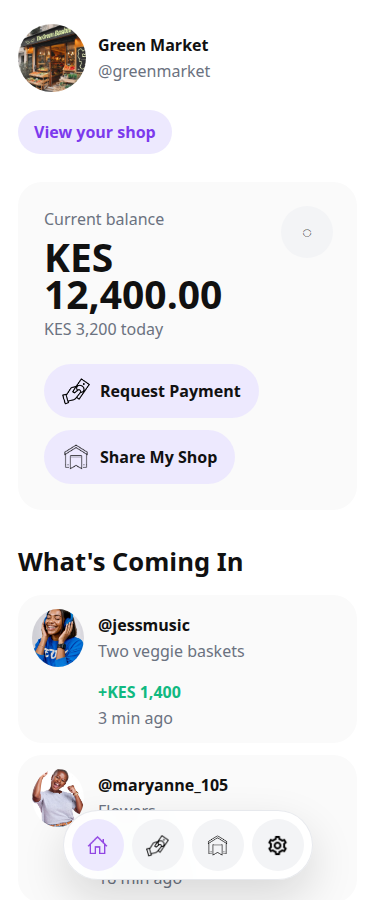
\includegraphics[height=0.78\textheight]{merchant_home_mobile.png}
    \caption{Merchant home page on mobile, showing earnings and incoming payment activity.}
    \label{fig:merchant-home}
\end{figure}

Figure~\ref{fig:merchant-home} shows the merchant view in the mobile-first context. The page gives a business owner immediate access to current balance, today's collection, request-payment actions and recent incoming payments.

\begin{figure}[H]
    \centering
    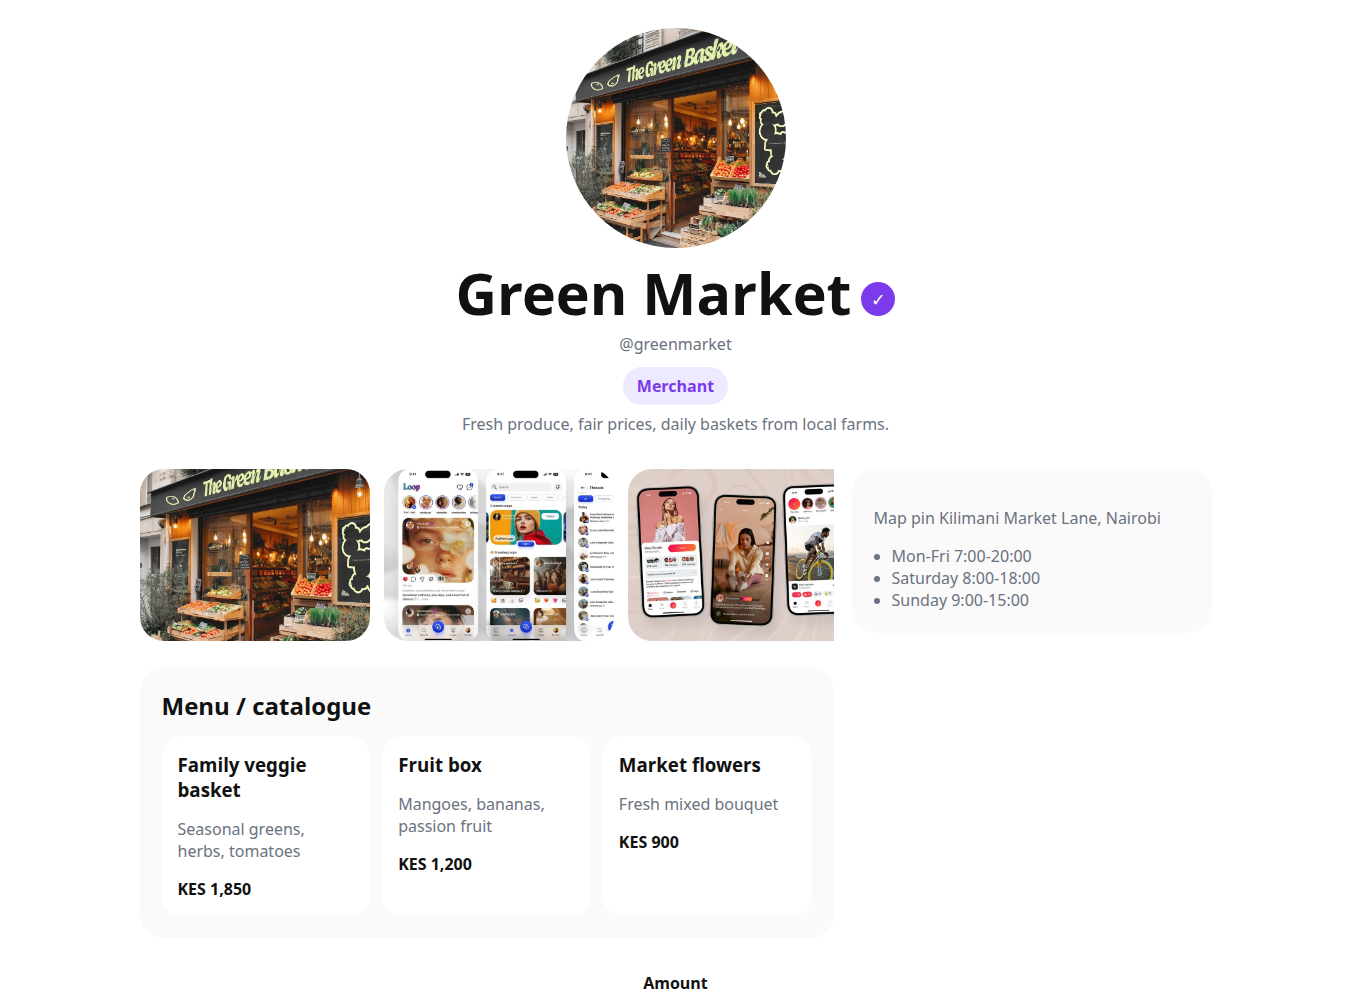
\includegraphics[width=\textwidth]{profile_laptop.png}
    \caption{Merchant profile and payment destination for @greenmarket.}
    \label{fig:profile}
\end{figure}

Figure~\ref{fig:profile} shows the combined profile and pay screen. For merchants, the profile carries storefront imagery, catalogue items, location, opening hours and a payment section. This aligns with the project goal of making merchants look like businesses rather than anonymous till numbers.

\subsection{Consistency}
The UI uses consistent visual rules across pages:
\begin{itemize}
    \item buttons are pill-shaped and respond to hover and click states;
    \item cards use large rounded corners;
    \item form inputs use rounded rectangular fields with purple focus rings;
    \item avatars are circular;
    \item primary calls to action use deep purple;
    \item secondary controls use soft purple or light gray.
\end{itemize}

This consistency helps the interface feel unified even though the customer and merchant flows have different personalities.

\subsection{Responsiveness}
The design is mobile-first but not mobile-only. The initial prototype had oversized text on laptop screens; the current pass introduces calmer laptop typography and more intentional desktop spacing. On mobile, the bottom navigation remains a floating capsule. On laptop, it becomes an in-flow capsule so it does not cover content while pages are being inspected.

\subsection{Accessibility and Usability}
The current prototype includes several accessibility-friendly choices: high contrast black text on white backgrounds, visible focus states on inputs, descriptive placeholder text, route-based navigation and readable touch targets. Areas that require further accessibility work include full keyboard testing, improved icon labels, form error announcements for screen readers and reduced-motion alternatives for users who prefer less animation.

\section{Database Design Analysis}

\subsection{Database Purpose}
Bloc's database must support identity, social transactions, merchant storefronts and payment routing. The central product decision is the @handle: every customer and merchant needs a unique human-readable identifier that can be used as a payment address and profile route.

\subsection{Core Entities}
The proposed database model includes the following entities:
\begin{longtable}{p{0.25\textwidth}p{0.65\textwidth}}
\toprule
\textbf{Entity} & \textbf{Purpose} \\
\midrule
User & Stores shared account information such as name, email, phone number, password hash, account type and verification status. \\
Handle & Stores unique @handle records and links each handle to a user or merchant account. \\
CustomerProfile & Stores customer biography, avatar, privacy settings and social-feed preferences. \\
MerchantProfile & Stores business name, category, bio, cover image, location, business hours and shop completeness status. \\
PaymentMethod & Stores payout routing details such as till number, paybill, account number or M-Pesa phone number. \\
Transaction & Stores amount, sender, receiver, timestamp, status, note, tag and payment rail reference. \\
Reaction & Stores optional social feedback attached to transactions, such as emojis or short reactions. \\
Product & Stores merchant catalogue items, descriptions, prices and media references. \\
MediaAsset & Stores image and file metadata for avatars, product photos, cover images and catalogue uploads. \\
\bottomrule
\end{longtable}

\subsection{Relationships}
The main relationships are:
\begin{itemize}
    \item one user owns one primary handle;
    \item one user has either a customer profile, a merchant profile, or both if account switching is enabled;
    \item one merchant profile has many products and media assets;
    \item one merchant profile has one active payout method;
    \item one transaction has one sender and one receiver;
    \item one transaction can have many reactions;
    \item handles are unique and should be indexed for fast search and payment lookup.
\end{itemize}

\subsection{Data Integrity and Security}
The database should enforce uniqueness on email, phone number and handle fields. Passwords must be stored as salted password hashes, never plain text. Payment method details should be encrypted or tokenized depending on backend infrastructure. Transaction records should be immutable except for status updates, because they represent financial history. Audit timestamps should be added to sensitive records such as payment methods and account settings.

\section{Code Design Analysis}

\subsection{Frontend Architecture}
The current frontend uses React with Vite and React Router. The code follows the modular structure specified in the Bloc design document:
\begin{itemize}
    \item each page lives in \texttt{src/pages/};
    \item each page has a matching stylesheet in \texttt{src/styles/};
    \item shared components live in \texttt{src/components/};
    \item shared mock data and asset imports live in \texttt{src/data/blocData.js};
    \item the bottom navigation is isolated in \texttt{src/components/BottomNav/}.
\end{itemize}

This separation supports maintainability because a developer can edit the merchant homepage without accidentally changing the customer signup page or profile screen.

\subsection{Routing}
The implemented routes are:
\begin{itemize}
    \item \texttt{/} -- signup and path selection;
    \item \texttt{/customer-login} -- customer onboarding;
    \item \texttt{/merchant-login} -- merchant onboarding and store setup;
    \item \texttt{/customer-home} -- customer dashboard;
    \item \texttt{/merchant-home} -- merchant dashboard;
    \item \texttt{/profile/:handle} -- profile and payment screen;
    \item \texttt{/settings} -- settings and account controls.
\end{itemize}

The router centralizes route ownership in \texttt{App.jsx}. This makes the navigation structure clear and easy to extend.

\subsection{Modularity}
The most important reusable component is \texttt{BottomNav}. It accepts a variant prop and renders a customer or merchant navigation capsule. It owns its own stylesheet, so page styles do not need to know how the component is implemented. This follows the design document rule that shared components must manage their own styling.

\subsection{Maintainability}
The codebase is maintainable because class names are page-prefixed, styles are isolated and data is centralized. Mock data is currently stored in one file so the prototype can be inspected without backend services. During backend integration, this data layer can be replaced by API calls without rewriting every page.

\subsection{Security Considerations}
The current frontend does not store real credentials or process real money. For production, the following controls will be required:
\begin{itemize}
    \item authenticated sessions using secure tokens;
    \item server-side validation for all signup and payment forms;
    \item encrypted payment-method storage;
    \item rate limiting on handle availability checks;
    \item role-based authorization for merchant-only settings;
    \item backend verification of transaction status from the payment rail.
\end{itemize}

\section{Integration of UI, Database and Code}

\subsection{Frontend-to-Backend Interaction}
The frontend will communicate with the backend through REST endpoints. Expected endpoints include authentication, handle availability, profile retrieval, merchant catalogue management, transaction initiation, transaction history and settings updates.

\subsection{Data Flow}
A typical customer payment flow is:
\begin{enumerate}
    \item the customer searches for a handle;
    \item the frontend requests the matching profile from the backend;
    \item the customer enters an amount and optional note;
    \item the backend validates the receiver, sender and payment amount;
    \item the backend initiates the M-Pesa STK Push or equivalent payment flow;
    \item the backend records a pending transaction;
    \item the payment provider callback updates the transaction status;
    \item the frontend displays the completed transaction in the social feed.
\end{enumerate}

\subsection{Error Handling}
Error handling should keep users in context. If signup fails, the form should preserve all entered values and display the error beside the relevant field. If payment initiation fails, the profile page should show a clear message and allow the user to retry without losing amount or note content. Network errors should be phrased in human language rather than exposing raw API messages.

\section{Recommendations}

\subsection{User Interface Improvements}
\begin{itemize}
    \item Add a dedicated search/pay page instead of routing search directly to a sample profile.
    \item Improve screen-reader labels for icon-only controls.
    \item Add reduced-motion support for users who disable animations.
    \item Add empty, loading and error states for every API-backed list.
    \item Add form progress indicators for the longer merchant signup flow.
\end{itemize}

\subsection{Database and Backend Improvements}
\begin{itemize}
    \item Create database migrations early so schema changes are tracked.
    \item Add unique indexes for handles, emails and phone numbers.
    \item Store transaction status history for auditability.
    \item Separate public profile data from private account data.
    \item Encrypt or tokenize payout method details.
\end{itemize}

\subsection{Code Improvements}
\begin{itemize}
    \item Add unit tests for form validation and route rendering.
    \item Add integration tests for customer and merchant onboarding flows.
    \item Replace mock data with service functions before backend integration.
    \item Introduce a small design-token file for repeated colors and radii.
    \item Add linting rules for accessibility where possible.
\end{itemize}

\section{Conclusion}
Bloc's current frontend prototype successfully communicates the product's core idea: payments can be social, expressive and human without abandoning the infrastructure Kenyans already trust. The strongest screens are the root page, customer onboarding, customer home, merchant mobile dashboard and merchant profile/payment page. These screens show a consistent visual language built around white space, rounded components, profile imagery and soft purple interaction states.

From a code perspective, the project now follows the intended modular structure: pages are isolated, styles are matched by page name, routing is centralized and the bottom navigation is a reusable component. From a database perspective, the most important future work is to model handles, profiles, transactions, merchant catalogues and payout methods in a secure and scalable way. The next implementation phase should connect the polished frontend to a backend API, enforce authentication, and integrate Safaricom Daraja for real payment routing.

\newpage
\section*{References}
\addcontentsline{toc}{section}{References}

\begin{enumerate}
    \item Bloc Design Document. (2026). \textit{Bloc Design Document: Version 1.0 -- Summer 2026}. Internal project specification.
    \item Nielsen, J. (1994). \textit{10 usability heuristics for user interface design}. Nielsen Norman Group.
    \item React. (2026). \textit{React documentation}. Meta Open Source.
    \item React Router. (2026). \textit{React Router documentation}. Remix Software.
    \item Safaricom PLC. (2026). \textit{Daraja API documentation}. Safaricom Developer Portal.
    \item Vite. (2026). \textit{Vite documentation}. VoidZero Inc.
    \item Wainaina, N. (2026). \textit{Bloc: A social-first unified payments platform for the Kenyan market}. SWE Midterm Project Report, United States International University -- Africa.
    \item World Wide Web Consortium. (2023). \textit{Web Content Accessibility Guidelines (WCAG) 2.2}. W3C.
\end{enumerate}

\end{document}
